\documentclass[12pt]{article}

% defining image path
\usepackage{graphicx}
\graphicspath{ {./images/} }

% tables
\usepackage[utf8]{inputenc}
\usepackage[table]{xcolor}
\usepackage{enumitem}
\setlist{nolistsep}

\pagestyle{empty}
\setcounter{secnumdepth}{2}

\topmargin=0cm
\oddsidemargin=0cm
\textheight=22.0cm
\textwidth=16cm
\parindent=0cm
\parskip=0.15cm
\topskip=0truecm
\raggedbottom
\abovedisplayskip=3mm
\belowdisplayskip=3mm
\abovedisplayshortskip=0mm
\belowdisplayshortskip=2mm
\normalbaselineskip=12pt
\normalbaselines


\begin{document}

\vspace*{0.5in}
\centerline{\bf\Large
Requirements for the Kakuro project}

\vspace*{0.5in}
\centerline{\bf\Large Iteration 1 COMP354}

\vspace*{0.5in}
\centerline{\bf\Large Team PK-A}

\vspace*{0.5in}
\centerline{\bf\Large 9 February 2020}

\vspace*{1.5in}
\begin{table}[htbp]
\caption{Team Members}
\begin{center}
\begin{tabular}{|c |c | c|}
\hline
Name & Role & ID Number \\
\hline\hline
Tiffany Ah King & Documenter & 40082976 \\
\hline
Isabelle Charette & Coder & 40008121 \\
\hline
Brian Gamboc-Javiniar & Documenter & 40033124 \\
\hline
Vsevolod Ivanov & Coder & 40004286 \\
\hline
Chang Liu & Documenter & 40056360 \\
\hline
Nolan Mckay & Documenter & 27873557 \\
\hline
Nalveer Moocheet & Coder & 40072605 \\
\hline
Hoang Thuan Pham & Documenter & 40022992 \\
\hline
Audrey-Laure St-Louis & Quality Control & 27558783 \\
\hline
Jia Ming Wei & Organizer & 40078192 \\
\hline
\end{tabular}
\end{center}
\end{table}


\newpage

\renewcommand*\contentsname{Table of Contents}

\tableofcontents

\newpage
\section{System}

\subsection{Purpose}

This Software Requirements Document describes the specifications of the Kakuro puzzle game, which is in partial fulfillment of the requirements of COMP 354 - Introduction to Software Engineering. It will define the requirements of user interfaces, user stories, game mechanics and how the software should work. The requirement analysis will include a use case diagrams and a domain model diagram to describe the problem domain of the application. It will also identifies non-functional requirements and hardware/software constraints. It also provides a glossary to formally describes key concepts involved in the project. This document is designed for Team Pk-A [1]. \\

There are three plannings to our project: software requirements, architectural and detailed design specification, and implementation. Following the due dates, we will complete our deliverables as listed below.

\begin{center}
\setlength{\tabcolsep}{20pt}
\renewcommand{\arraystretch}{2}
\begin{tabular}{ |p{4cm}|p{4cm}|p{4cm}| }
\hline
Project Plan & Deliverable & Date \\
\hline
Software requirements specification & A requirements document & Sunday 9 February 2020 \\ 
\hline
Architectural and detailed design specification & A design document & Sunday 15 March 2020 \\ 
\hline
Implementation & Test plan, report, and final game & Sunday 5 April 2020 \\ 
\hline
\end{tabular}
\end{center}
 
\subsection{Context}

The software we are building is a requirement for our Introduction to Software Engineering course to show our acquired knowledge for software development. The requirements to the maintenance of the software will be taken into account as these are the fundamentals of development. We will be interchanging roles for three iterations and to expose ourselves to different kind of view points of expertise in the field.

\subsection{Business Goals}

The business objective of this project is to design and implement a single-player desktop game Kukuro based on the popular puzzle game of the same name. The application will enforce the rules of a classical Kukuro game and it will allow a single player to play a random 10x10 Kakuro game on a personal computer. Additionally, players can register, save a game in progress, resume a saved game and view their best game record.

\newpage

\section{Domain Concepts}

The domain model of the Kakuro application consists of players, games, cells, game progresses and saved white cells. A player can play one game at a time. Each game contains cells. There are two types of cells. Black cells represent non-fillable cells. Some of them contain clues about the puzzle to which it belongs. White cells are cells in which players can enter a number from 1 to 9 inclusively. A player can also save a game that is currently being played. The saved game progress includes the elapsed time, and any prior input that the player has entered. 

\begin{figure}[htbp]
    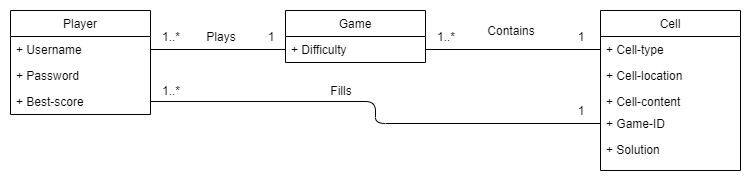
\includegraphics[width=1\textwidth]{DomainModel}
    \caption{Domain Model of the Kakuro Game System}
    \label{fig:DomainModel}
\end{figure}

\newpage

\section{Actors} 

Players are the only actors for this application. They are users who can play the game. They can register and login. Moreover, they can interact with the graphical user interface by starting the game, viewing overall scores of other players, as well as their personal scores. Finally, they have the ability to choose the difficulty, pause and resume a game when they need to. 
As this is only the first iteration, the players are currently `anonymous` users, therefore anyone can play the game without registering.

\newpage

\section{Use Cases}

\subsection{Overview}
Our use case diagram represents the use cases and features that we will be implementing for the Kukuro game. As an actor, players can normally start the game, pause, resume, or restart. Furthermore, they are able to save their progress and load it at any point of time. Also, the player is able to view other player's high-score, as well as choosing the level of difficulty.

\begin{figure}[htbp]
    \centering
    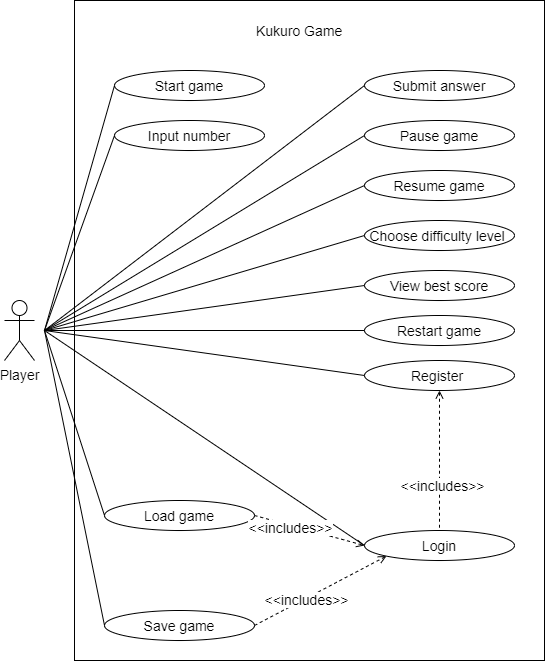
\includegraphics[scale=0.6]{UseCaseDiagram}
    \caption{Use Case Diagram}
    \label{fig:UseCaseDiagram}
\end{figure}

\newpage

%%%%%%%%%%%%%%%%%%%%%%%%%%%%% USE CASE 1 

\subsection{Use Case 1 - Start game} 

\begin{center}
\setlength{\tabcolsep}{18pt}
\renewcommand{\arraystretch}{1.1}
\begin{tabular}{ |p{3.4cm}|p{10cm}| }
    \hline
    \textbf{Item} & \textbf{Description} \\
    \hline
    Name & Start game \\
    \hline
    Summary & A player starts a game \\
    \hline
    Actors & Player \\
    \hline
    Precondition &  
    \vspace*{-0.1in}
    \begin{enumerate}[leftmargin=0.2in]
    \item The application is running
    \item No game is in progress
    \end{enumerate}  \\
    \hline
    Main Scenario &     
    \vspace*{-0.1in}
    \begin{enumerate}[leftmargin=0.2in]
    \item The player clicks on the start button
    \item A new Kakuro game is displayed
    \item The timer starts
    \end{enumerate}  \\
    \hline
    Alternate Scenario & None  \\
    \hline
    Exceptions & None \\
    \hline
    Postcondition & 
    \vspace*{-0.1in}
    \begin{enumerate}[leftmargin=0.2in]
    \item A new Kakuro game is displayed 
    \end{enumerate}  \\
    \hline
    Priority & High  \\
    \hline
    \small{Traces to Test Cases} & 
    Current unit test(s): \textbf{TestBoardUI, TestBoard} \newline
    Please refer to it below
    \\
    \hline
\end{tabular}
\end{center}

\textbf{TestBoardUI - testBoardUIGeneration()} 
    
\textit{Description:} \newline
The board's user interface is generated \newline

\textit{Input:} \newline
Takes an integer number for rows and columns, 3 and 5 respectively. \newline 

\textit{Expected results:} \newline
The desktop application game can be seen and ready to be played with the given rows and columns. \newline
\\

\textbf{TestBoard - testSize()} 
    
\textit{Description:} \newline
The board has a size \newline

\textit{Input:} \newline
Takes an integer number of 10 for both rows and columns. \newline 

\textit{Expected results:} \newline
The game has a size with the given rows and columns. \newline
\\

\newpage

%%%%%%%%%%%%%%%%%%%%%%%%%%%%% USE CASE 2 

\subsection{Use Case 2 - Submit answer}

\begin{center}
\setlength{\tabcolsep}{16pt}
\renewcommand{\arraystretch}{1.1}
\begin{tabular}{ |p{3.4cm}|p{10cm}| }
    \hline
    \textbf{Item} & \textbf{Description} \\
    \hline
    Name & Submit answer \\
    \hline
    Summary & A player checks whether the entered numbers are a solution to the puzzle \\
    \hline
    Actors & Player \\
    \hline
    Precondition & 
    \vspace*{-0.1in}
    \begin{enumerate}[leftmargin=0.2in]
    \item A game is in progress
    \item All white cells are filled
    \end{enumerate}  \\
    \hline
    Main Scenario &     
    \vspace*{-0.1in}
    \begin{enumerate}[leftmargin=0.2in]
    \item The player clicks on the submit button
    \item The application validates the answer and the answer is correct
    \item The timer stops and time is shown
    \item A message is displayed, informing the player that the answer was correct
    \item The game ends
    \end{enumerate}  \\
    \hline
    Alternate Scenario & 
    \vspace*{-0.1in}
    \begin{enumerate}[leftmargin=0.2in]
    \item The player clicks on the submit button
    \item The application validates the answer and the answer is wrong
    \item A message is displayed, informing the player that the answer was incorrect
    \item The game resumes
    \end{enumerate}  \\
    \hline
    Exceptions &  None \\
    \hline
    Postcondition & None \\
    \hline
    Priority & High  \\
    \hline
    \small{Traces to Test Cases} & Current unit test(s): \textbf{TestBoard} \newline
    Please refer to it below  
    \\
    \hline
\end{tabular}
\end{center}

\textbf{TestBoard - testValidBoard()} 
    
\textit{Description:} \newline
Validating if the board does not accept the inputs as a solved solution.  \newline

\textit{Input:} \newline
Valid inputs are being put in the board. \newline 

\textit{Expected results:} \newline
The input values solved the board, which returns true. \newline
\\

\textbf{TestBoard - testNotValidBoardOneSumIsWrong()} 
    
\textit{Description:} \newline
Validating if the board does not accept the inputs as a solved solution.  \newline

\textit{Input:} \newline
Invalid inputs are being put in the board. \newline 

\textit{Expected results:} \newline
The input values does not solve the board, which returns false. \newline
\\

\textbf{TestBoard - testNotValidBoardCorrectSumDuplicateEntries()} 
    
\textit{Description:} \newline
Validating if the board does not accept duplicate entries in the same row or column  \newline

\textit{Input:} \newline
Duplicate inputs are being put in the board. \newline 

\textit{Expected results:} \newline
The input values does not solve the board, which returns false. \newline
\\

\newpage

%%%%%%%%%%%%%%%%%%%%%%%%%%%%% USE CASE 3

\subsection{Use Case 3 - Restart game}

\begin{center}
\setlength{\tabcolsep}{18pt}
\renewcommand{\arraystretch}{1.3}
\begin{tabular}{ |p{3.4cm}|p{10cm}| }
    \hline
    
   \textbf{Item} & \textbf{Description} \\
    \hline
    Name & Restart game \\
    \hline
    Summary & The game restarts the current game. All the white cells will be returned to empty and the timer will reset \\
    \hline
    Actors & Player \\
    \hline
    Precondition & A game is in progress \\
    \hline
    Main Scenario &     
    \vspace*{-0.1in}
    \begin{enumerate}[leftmargin=0.2in]
    \item The player selects restart game
    \item A confirmation message is shown
    \item The player confirms restarting the game
    \item All white cells are cleared
    \item Timer resets
    \end{enumerate}  \\
    \hline
    Alternate Scenario & \vspace*{-0.1in}
    \begin{enumerate}[leftmargin=0.2in]
    \item The player declines to restart the game
    \item The confirmation message disappears
    \item The game resumes
    \end{enumerate}  \\
    \hline
    Exceptions &  None\\
    \hline
    Postcondition & 
    \vspace*{-0.1in}
    \begin{enumerate}[leftmargin=0.2in]
        \item The same game begins from the start.
    \end{enumerate}  \\
    \hline
    Priority & Medium  \\
    \hline
    \small{Traces to Test Cases} & Add when test cases done  \\
    \hline
\end{tabular}
\end{center}

\newpage

%%%%%%%%%%%%%%%%%%%%%%%%%%%%% USE CASE 4 - Choose difficulty level

\subsection{Use Case 4 - Choose difficulty level} 

\begin{center}
\setlength{\tabcolsep}{18pt}
\renewcommand{\arraystretch}{1.3}
\begin{tabular}{ |p{3.4cm}|p{10cm}| }
    \hline
   \textbf{Item} & \textbf{Description} \\
    \hline
    Name & Choose difficulty level \\
    \hline
    Summary & A player chooses a difficulty level (Easy - Medium - Hard) for the next game \\
    \hline
    Actors & Player \\
    \hline
    Precondition & 
    None \\
    \hline
    Main Scenario &     
    \vspace*{-0.1in}
    \begin{enumerate}[leftmargin=0.2in]
        \item The player clicks on the difficulty button
        \item A list of different difficulties (Easy - Medium - Hard) is displayed
        \item The player selects a difficulty level 
        \item The list disappears
        \item The selected difficulty is displayed to the player
    \end{enumerate}  \\
    \hline
    Alternate Scenario & None \\
    \hline
    Exceptions &  None\\
    \hline
    Postcondition & 
    \vspace*{-0.1in}
    \begin{enumerate}[leftmargin=0.2in]
        \item The system saves the player difficulty preference
    \end{enumerate}  \\
    \hline
    Priority & Low  \\
    \hline
    \small{Traces to Test Cases} & Add when test cases done  \\
    \hline
\end{tabular}
\end{center}

\newpage

%%%%%%%%%%%%%%%%%%%%%%%%%%%%% USE CASE 5 - Input number

\subsection{Use Case 5 - Input number}

\begin{center}
\setlength{\tabcolsep}{18pt}
\renewcommand{\arraystretch}{1.3}
\begin{tabular}{ |p{3.4cm}|p{12cm}| }
    \hline
    \textbf{Item} & \textbf{Description} \\
    \hline
    Name & Input number \\
    \hline
    Summary & The player chooses a white cell and enters a number from 1 to 9 (inclusive) \\
    \hline
    Actors & Player \\
    \hline
    Precondition & 
    \vspace*{-0.1in}
    \begin{enumerate}[leftmargin=0.2in]
        \item A game that is in progress.
    \end{enumerate}  \\
    \hline
    Main Scenario &     
    \vspace*{-0.1in}
    \begin{enumerate}[leftmargin=0.2in]
        \item The player chooses a white cell that is empty
        \item The player enters a number between 0-9
        \item The number chosen by the player is shown in the white cell
    \end{enumerate}  \\
    \hline
    Alternate Scenario &     
    \vspace*{-0.1in}
    \begin{enumerate}[leftmargin=0.2in]
        \item The player chooses a white cell that is already filled
        \item The player enters a number between 0-9
        \item The number previously shown in the cell is removed and the new selected number is shown in the cell
    \end{enumerate}  \\
    \hline
    Exceptions & 
    \vspace*{-0.1in}
    \begin{enumerate}[leftmargin=0.2in]
        \item The player chooses a black cell 
        \item The player enters a letter
    \end{enumerate}  \\
    \hline
   Postcondition & 
    \vspace*{-0.1in}
    \begin{enumerate}[leftmargin=0.2in]
        \item The chosen number entered by the player is shown in the selected cell 
    \end{enumerate} \\
    \hline
    Priority & High  \\
    \hline
    \small{Traces to Test Cases} & Current unit test(s): \textbf{TestBoardCell, TestGameViewInput} 
    \newline
    Please refer to it below  
    \\
    \hline
\end{tabular}
\end{center}

\textbf{TestBoardCell - testNonInputCell()} \\

\textit{Description:} \newline
Verify that non-input cells are EMPTY cells \newline

\textit{Input:} \newline
Using a EMPTY cell type as a board cell \newline 

\textit{Expected results:} \newline
The non-input cells is an EMPTY cell, which is truthy.
\newline
\\

\textbf{TestBoardCell - testInputCell()} \\

\textit{Description:} \newline
Verify a cell's first value has the correct input, as well as being an EMPTY cell. \newline

\textit{Input:} \newline
Populates a cell's first value with an integer. \newline 

\textit{Expected results:} \newline
The EMPTY cell is truthy and has a first value. \newline
\\

\textbf{TestBoardCell - testInputAnswerCell()} \\

\textit{Description:} \newline
Verify that a cell type is EMPTY with a left and right number. \newline

\textit{Input:} \newline
Passing two numbers with an EMPTY cell. \newline 

\textit{Expected results:} \newline
The EMPTY cell has two integer values. \newline
\\

\textbf{TestGameViewInput - testValidInputNumber()} 
    
\textit{Description:} \newline
Validating the input number is a valid number from 1-9.  \newline

\textit{Input:} \newline
Input values are from 1-9. \newline 

\textit{Expected results:} \newline
The valid inputs are truthy as it ranges from 1-9. \newline
\\

\textbf{TestGameViewInput - testValidInputNumber()} 
    
\textit{Description:} \newline
Validating the input number is an invalid number which is not from 1-9.  \newline

\textit{Input:} \newline
Input values is a string. \newline 

\textit{Expected results:} \newline
The input values are falsy as it is not wihin the 1-9 range. \newline
\\

\textbf{TestGameViewInput - testInvalidInputString()} 
    
\textit{Description:} \newline
Validating the input number is an invalid number which is not from 1-9, but a string  \newline

\textit{Input:} \newline
Input values is a string. \newline 

\textit{Expected results:} \newline
The input values are falsy as it is not a integer. \newline
\\

\newpage

%%%%%%%%%%%%%%%%%%%%%%%%%%%%% USE CASE 6 - Pause game

\subsection{Use Case 6 - Pause game}

\begin{center}
\setlength{\tabcolsep}{18pt}
\renewcommand{\arraystretch}{1.3}
\begin{tabular}{ |p{3.4cm}|p{10cm}| }
    \hline
    \textbf{Item} & \textbf{Description} \\
    \hline
    Name & Pause game \\
    \hline
    Summary & The player pauses the game their currently playing \\
    \hline
    Actors & Player \\
    \hline
    Precondition & 
    \vspace*{-0.1in}
    \begin{enumerate}[leftmargin=0.2in]
        \item A game that is in progress.
    \end{enumerate}  \\
    \hline
    Main Scenario &     
    \vspace*{-0.1in}
    \begin{enumerate}[leftmargin=0.2in]
        \item The player clicks on the pause button
        \item The game board is blurred, preventing the player from playing
        \item The timer stops  
        \item The application informs the player that the game is paused
    \end{enumerate}  \\
    \hline
    Alternate Scenario & None \\
    \hline
    Exceptions & None \\
    \hline
    Postcondition & \vspace*{-0.1in}
    \begin{enumerate}[leftmargin=0.2in]
        \item The game is paused
    \end{enumerate}  \\
    \hline
    Priority & Medium  \\
    \hline
    \small{Traces to Test Cases} & Current unit test(s): \textbf{TestChrono} 
    \newline
    Please refer to it below  
    \\
    \hline
\end{tabular}
\end{center}

\textbf{TestChrono - testRunStopChronoAfter3Seconds()} 
    
\textit{Description:} \newline
Verify the pause stops the timer. \newline

\textit{Input:} \newline
Presses the pause button to stop the timer for incrementing. \newline 

\textit{Expected results:} \newline
Asserts that the timer was paused after 3 seconds. \newline
\\

\newpage

%%%%%%%%%%%%%%%%%%%%%%%%%%%%% USE CASE 7 - Resume game

\subsection{Use Case 7 - Resume game}

\begin{center}
\setlength{\tabcolsep}{18pt}
\renewcommand{\arraystretch}{1.3}
\begin{tabular}{ |p{3.4cm}|p{10cm}| }
    \hline
    \textbf{Item} & \textbf{Description} \\
    \hline
    Name & Resume game \\
    \hline
    Summary & The player resumes a game that is currently being paused \\
    \hline
    Actors & Player \\
    \hline
    Precondition & 
    \vspace*{-0.1in}
    \begin{enumerate}[leftmargin=0.2in]
        \item A game that is paused
    \end{enumerate}  \\
    \hline
    Main Scenario &     
    \vspace*{-0.1in}
    \begin{enumerate}[leftmargin=0.2in]
        \item The player clicks on the resume button
        \item The game board is unblurred and revealed to the user
        \item The timer starts ticking again
    \end{enumerate}  \\
    \hline
    Alternate Scenario & None \\
    \hline
    Exceptions & None \\
    \hline
    Postcondition & \vspace*{-0.1in}
    \begin{enumerate}[leftmargin=0.2in]
        \item The game is resumed and the player can continue playing
    \end{enumerate}  \\
    \hline
    Priority & Medium  \\
    \hline
    \small{Traces to Test Cases} & Add when test cases done  \\
    \hline
\end{tabular}
\end{center}

\newpage

%%%%%%%%%%%%%%%%%%%%%%%%%%%%% USE CASE 8 - Login

\subsection{Use Case 8 - Login}

\begin{center}
\setlength{\tabcolsep}{18pt}
\renewcommand{\arraystretch}{1.3}
\begin{tabular}{ |p{3.4cm}|p{10cm}| }
    \hline
    
   \textbf{Item} & \textbf{Description} \\
    \hline
    Name & Login \\
    \hline
    Summary & The player signs into their game account \\
    \hline
    Actors & Player \\
    \hline
    Precondition & None \\
    \hline
    Main Scenario &     
    \vspace*{-0.1in}
    \begin{enumerate}[leftmargin=0.2in]
        \item The player provides a username and a password
        \item The application authenticates the user
    
       
    \end{enumerate}  \\
    \hline
    Alternate Scenario & None \\
    \hline
    Exceptions & 
    \vspace*{-0.1in}
    \begin{enumerate}[leftmargin=0.2in]
        \item The player enters an invalid username or password
        \item The application informs the player that login was unsuccessful
    \end{enumerate}  \\
    \hline
    Postcondition & None \\
    \hline
    Priority & Low  \\
    \hline
    \small{Traces to Test Cases} & Add when test cases done  \\
    \hline
\end{tabular}
\end{center}

\newpage

%%%%%%%%%%%%%%%%%%%%%%%%%%%%% USE CASE 9 - Register player

\subsection{Use Case 9 - Register}

\begin{center}
\setlength{\tabcolsep}{18pt}
\renewcommand{\arraystretch}{1.3}
\begin{tabular}{ |p{3.4cm}|p{10cm}| }
    \hline
    
\textbf{Item} & \textbf{Description} \\
    \hline
    Name & Register\\
    \hline
    Summary & The player registers and makes their account \\
    \hline
    Actors & Player \\
    \hline
    Precondition & 
    \vspace*{-0.1in}
    \begin{enumerate}[leftmargin=0.2in]
        \item The application is running
    \end{enumerate}  \\
    \hline
    Main Scenario &     
    \vspace*{-0.1in}
    \begin{enumerate}[leftmargin=0.2in]
        \item The player clicks the register button
        \item The player registers by inputting username and password
        \item The player gets their own account
    \end{enumerate} \\
    \hline
    Alternate Scenario & None \\
    \hline
    Exceptions & 
    \vspace*{-0.1in}
    \begin{enumerate}[leftmargin=0.2in]
        \item The username that the player entered already exists
        \item The second password input doesn't match the first one
        \item Username and password are too weak
    \end{enumerate}  \\
    \hline
    Postcondition &
    \vspace*{-0.1in}
    \begin{enumerate}[leftmargin=0.2in]
        \item The account is registered
    \end{enumerate}  \\
    \hline
    Priority & Low \\
    \hline
    \small{Traces to Test Cases} & Add when test cases done  \\
    \hline
\end{tabular}
\end{center}

\newpage

%%%%%%%%%%%%%%%%%%%%%%%%%%%%% USE CASE 10 - Save game

\subsection{Use Case 10 - Save game}

\begin{center}
\setlength{\tabcolsep}{18pt}
\renewcommand{\arraystretch}{1.3}
\begin{tabular}{ |p{3.4cm}|p{10cm}| }
    \hline
    \textbf{Item} & \textbf{Description}\\
    \hline
    Name & Save game \\
    \hline
    Summary & A player saves the game that is currently being played \\
    \hline
    Actors & Player \\
    \hline
    Precondition & 
    \vspace*{-0.1in}
    \begin{enumerate}[leftmargin=0.2in]
        \item The player has logged in
        \item A game is in progress.
        
    \end{enumerate}  \\
    \hline
    Main Scenario &     
    \vspace*{-0.1in}
    \begin{enumerate}[leftmargin=0.2in]
        \item The player pressed the save button
        \item The current progress (time and inputs) is saved in player's account
        \item The game quits
    \end{enumerate}  \\
    \hline
    Alternate Scenario & None \\
    \hline
    Exceptions & None  \\
    \hline
    Postcondition &
    \vspace*{-0.1in}
    \begin{enumerate}[leftmargin=0.2in]
        \item The progress of the game played by the player is saved
        \item The game quits
    \end{enumerate}  \\
    \hline
    Priority & Low \\
    \hline
    \small{Traces to Test Cases} & Add when test cases done  \\
    \hline
\end{tabular}
\end{center}

\newpage

%%%%%%%%%%%%%%%%%%%%%%%%%%%%% USE CASE 11 - Load the game

\subsection{Use Case 11 - Load game}

\begin{center}
\setlength{\tabcolsep}{18pt}
\renewcommand{\arraystretch}{1.3}
\begin{tabular}{ |p{3.4cm}|p{10cm}| }
    \hline
   \textbf{Item} & \textbf{Description} \\
    \hline
    Name & Load game \\
    \hline
    Summary & A player loads a saved game \\
    \hline
    Actors & Player \\
    \hline
    Precondition & 
    \vspace*{-0.1in}
    \begin{enumerate}[leftmargin=0.2in]
        \item The player has logged in
        \item There exists a game previously saved by the player
    \end{enumerate}  \\
    \hline
    Main Scenario & 
    \vspace*{-0.1in}
    \begin{enumerate}[leftmargin=0.2in]
    \item The player clicks on the load button 
    \item The system checks that the player has saved a game previously
    \item The game that the player was playing previously is displayed. All white cells which were filled by the player when the game was saved are filled with the same value
    \end{enumerate}  \\
     \hline
    Alternate Scenario & None  \\
    \hline
    Exceptions & None \\
    \hline
    Postcondition & 
    \vspace*{-0.1in}
    \begin{enumerate}[leftmargin=0.2in]
        \item The game that the player previously saved is loaded
    \end{enumerate} \\
    \hline
    Priority & Low \\
    \hline
    \small{Traces to Test Cases} & Add when test cases done  \\
    \hline
\end{tabular}
\end{center}

\newpage

%%%%%%%%%%%%%%%%%%%%%%%%%%%%% USE CASE 12 - View the best score

\subsection{Use Case 12 - View best score}

\begin{center}
\setlength{\tabcolsep}{18pt}
\renewcommand{\arraystretch}{1.3}
\begin{tabular}{ |p{3.4cm}|p{10cm}| }
    \hline
   \textbf{Item} & \textbf{Description} \\
    \hline
    Name & View best score \\
    \hline
    Summary & A player can view the best score. The scoreboard displays the top 10 fastest players and the time for each of them to complete a game. \\
    \hline
    Actors & Player \\
    \hline
    Precondition & 
    \vspace*{-0.1in}
    \begin{enumerate}[leftmargin=0.2in]
     
        \item No game is in progress
        
    \end{enumerate}  \\
    \hline
    Main Scenario & 
    \vspace*{-0.1in}
    \begin{enumerate}[leftmargin=0.2in]
        \item The player pressed the view best score button
        \item The scoreboard is displayed 
        \item The player views the scoreboard which displays the top 10 fastest players and the time for each of them to complete a game
        \item The user closes the scoreboard
       
    \end{enumerate}  \\
    \hline
    Alternate Scenario & None \\
    \hline
    Exceptions & None \\
    \hline
    Postcondition & None \\
    \hline
    Priority & Low \\
    \hline
    \small{Traces to Test Cases} & Add when test cases done  \\
    \hline
\end{tabular}
\end{center}

\newpage

\section{Non-Functional Constraints}

\subsection{Business Constraints - Game Mechanism}

The business constraints for the application is that it must enforce the rules of a classic Kakuro game. In Kakuro, each puzzle consists of black cells with clues that need to be solved by the empty white cells. The objective is to fill all empty white cells using numbers from 1 to 9. Each number can only used once for a clue in both vertical and horizontal white cells. The sum of each horizontal black cell must equal the clue on its left. Similarly the sum of each vertical cell must equal the clue on its right [2].

\subsection{Software Requirements}
The application constraints consist of making Kakuro a standalone java application, which can launched in any operating system due to the compilation being in the Java Virtual Machine (JVM). Secondly, the software must be built using Java Swing as a Graphical User Interface (GUI), and finally, it should have a database that runs in SQLite [3].

\vspace{5mm}

The work environment constraints restrict the application to be written in Java with JUnit for unit testing. Diagrams and especially Unified Modeling Language (UML) to be drawn in draw.io. Coupled with GitHub as our software repository and git as version control. Finally, all documentation must be written in Latex [3]. 
 

\subsection{Non-Functional Requirements}
 
\textbf{Reliability}: It is vital that the Kakuro game is error-free to provide a smooth and satisfying game play experience to players.

\vspace{5mm}

\textbf{Maintainability}: The design of the Kakuro application will be in a modular form which will allow many developers to work on different modules simultaneously and shorten debugging time. The modules should be designed in such a way that reduces coupling and dependencies. Code should be documented clearly and concisely to support knowledge transfer.

\vspace{5mm}

\textbf{Usability}: The graphical user must be pleasant to the eye, organized and intuitive to
use. This will encourage the user to play and improve user experience overall. 

\newpage

%%%%%%%%%%%%%%%%%%%%%%%%%%%%%%%%%%%

\section{User Interface}

The user interface of the Kakuro game application should be easy to use. It is the bridge connecting players and the application. A user friendly interface allows easy navigation through the game and improves players' overall experience. The user interface should be intuitive to players and helps them complete the game successfully.

When the application starts, the first thing shown to the players is a start menu. The menu includes buttons that allow players to start playing a Kakuro game, quit the application, register for an account and login to an existing account. Figure 3 describes a prototype proposed for the user interface of the start menu. 

\begin{figure}[htbp]
    \centering
    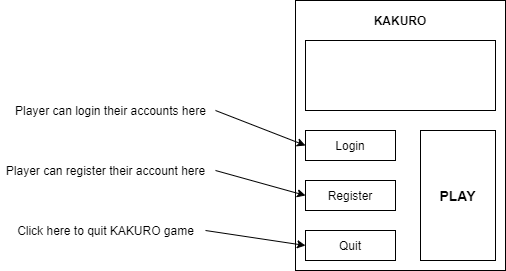
\includegraphics[scale=0.8]{UI-1.png}
    \caption{Kakuro Start Menu}
    \label{fig:UI-1}
\end{figure}

\newpage
After clicking on the play button, a game will begin. Figure 4 proposes a prototype for the gameplay user interface. In this interface, the black cells represent non-fillable cells. Black cells that have bars contain clues. The clues situate on the left or right of the bar. They hint the players for the sum of the corresponding column or row. The white cells are empty slots, where a number from 1 to 9 can be entered in each cell by the player. The interface also contains buttons to pause the game, submit the answer, and save the current game. 

\begin{figure}[htbp]
    \centering
    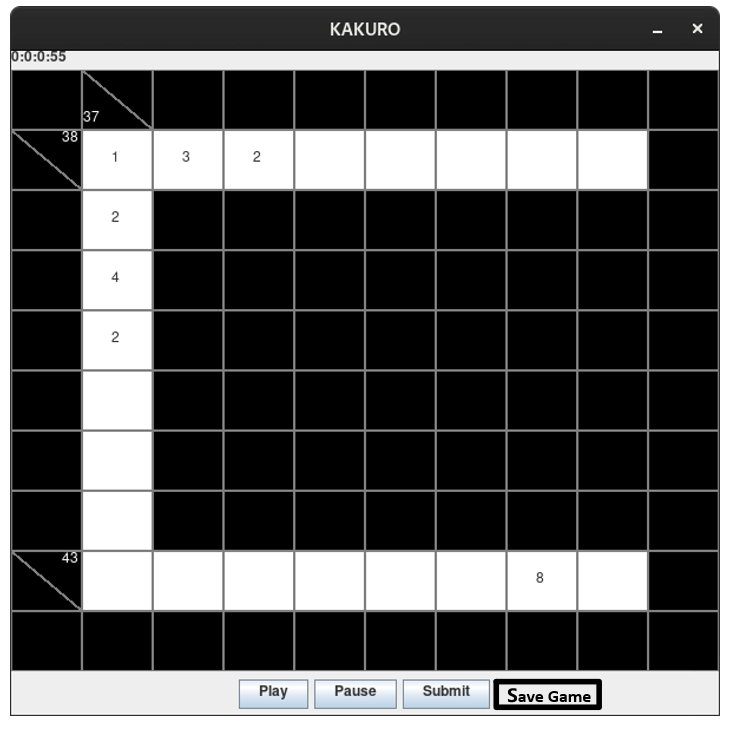
\includegraphics[scale=0.5]{UI-0.png}
    \caption{Game Board}
    \label{fig:UI-0}
\end{figure}

\newpage
When the player submits a correct attempt, a menu is displayed informing the player that the game is completed successfully. Now the player can view the best play records, restart the game, or quit the game by clicking on the corresponding button. Figure 5 describes the game completed interface.   

\begin{figure}[htbp]
    \centering
    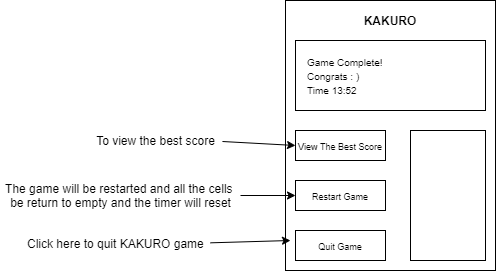
\includegraphics[scale=0.8]{UI-2.png}
    \caption{Game complete Interface}
    \label{fig:UI-2}
\end{figure}

\newpage
When a wrong solution is submitted the game will display that the solution was incorrect. The player will then have the option to resume the game and try again, restart the game or quit the game. Figure 6 describes the menu when a wrong solution is displayed. 


\begin{figure}[htbp]
    \centering
    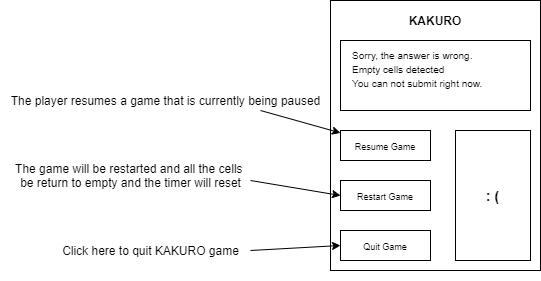
\includegraphics[scale=0.8]{UI-3.png}
    \caption{Wrong Answer Interface}
    \label{fig:UI-3}

\end{figure}

Figure 7 describes what the scoreboard will look like. The player will be able to look through the list of 10 fastest players and their best records. The scoreboard will consist of usernames and the associated times.

\begin{figure}[htbp]
    \centering
    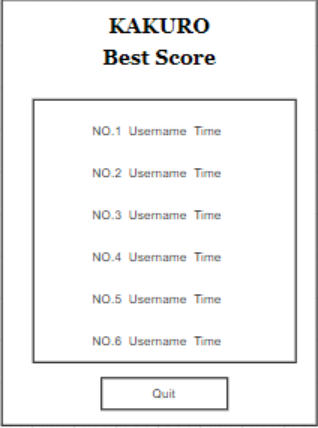
\includegraphics[scale=0.8]{UI-4.png}
    \caption{Top Times}
    \label{fig:UI-4}
\end{figure}



\newpage

\section{Glossary}

\textbf{Account}\\
The account is a record relating to the player. It will contain the saved game progress of the player. When the player will logins in, they will have access to their data.
\vspace{5mm}

\textbf{Best score}\\ 
High score consist of personal or overall scores of players based on how fast they completed the game.
\vspace{5mm}

\textbf{Clue} \\
A clue is a number displayed in a black cell. The clue hints players about the total sum of a row or column. 
\vspace{5mm}

\textbf{Cell} \\
A cell is either a black cell or a white cell. A black cell contains 'clues' that situates on the left or right of the backslash. The white cell are empty slots, where numbers are placed.
\vspace{5mm}

\textbf{Database}\\
A data storage that organized and keep information that runs on SQLite.
\vspace{5mm}

\textbf{Game}\\
It is a round of the Kakuro game. The player will launch it and play. The game end when the player submits  their answer
\vspace{5mm}

\textbf{Game Progress}\\
The state of the game that the player saved. It contains the amount of time that has passed and all the numbers that the user entered.
\vspace{5mm}

\textbf{Grid}\\
The grid will have a static size of 10x10, which consist of white and black cells. The black cells fills the first row and first column entirely.
\vspace{5mm}

\textbf{Player}\\
Player is the user that will engage in the game and interact with the interface.
\vspace{5mm}

\textbf{Solution}\\
A solution is the correct answer to a Kakuro puzzle. A solution consists of a specific combination of numbers with specific positions in the puzzle. For our Kakuro application, there is a unique solution to each game.
\vspace{5mm}

\textbf{Saved White Cell}\\
A saved white cell stores the player's input from a saved game.
\vspace{5mm}

\textbf{Timer or Time}\\
A timer represents the number of times left to complete the game before losing the score.
\vspace{5mm}

\newpage

\section{References}
\vspace{5mm}
  
[1] Team Redmond, Monopoly - Project Analysis and Development Plan Version 1.3\\
https://users.encs.concordia.ca/~paquet/wiki/images/6/67/Phase1final.pdf (Accessed: February 9, 2020)

[2] Wikipedia, Kakuro\\
https://en.wikipedia.org/wiki/Kakuro (Accessed:  February 9, 2020)

[3] Gregory Butler, Term Team Project Description
Kakuro\\ 
https://users.encs.concordia.ca/~gregb/home/PDF/comp354\_w2020\_project\_description.pdf (Accessed: February 9, 2020)\\

\setlength{\parindent}{10ex}

\newpage

\section{Description of File Format}

\subsection{.java}
File extension for Java code. The java files contains development `Java` code, where it will be compiled to `.class`.
\subsection{.tex}
File extension for Latex. All written `words` that are formatted in latex will be converted to produce a quality text format file in PDF.
\subsection{.jar}
File extension for Java executable. The game application will be distributed as a jar file. In order to start the application, the jar file associate with the application must be run.

\end{document}

